\appendix

\section{Appendix}

\subsection{Sonarcube report}\label{sonarcube-report}

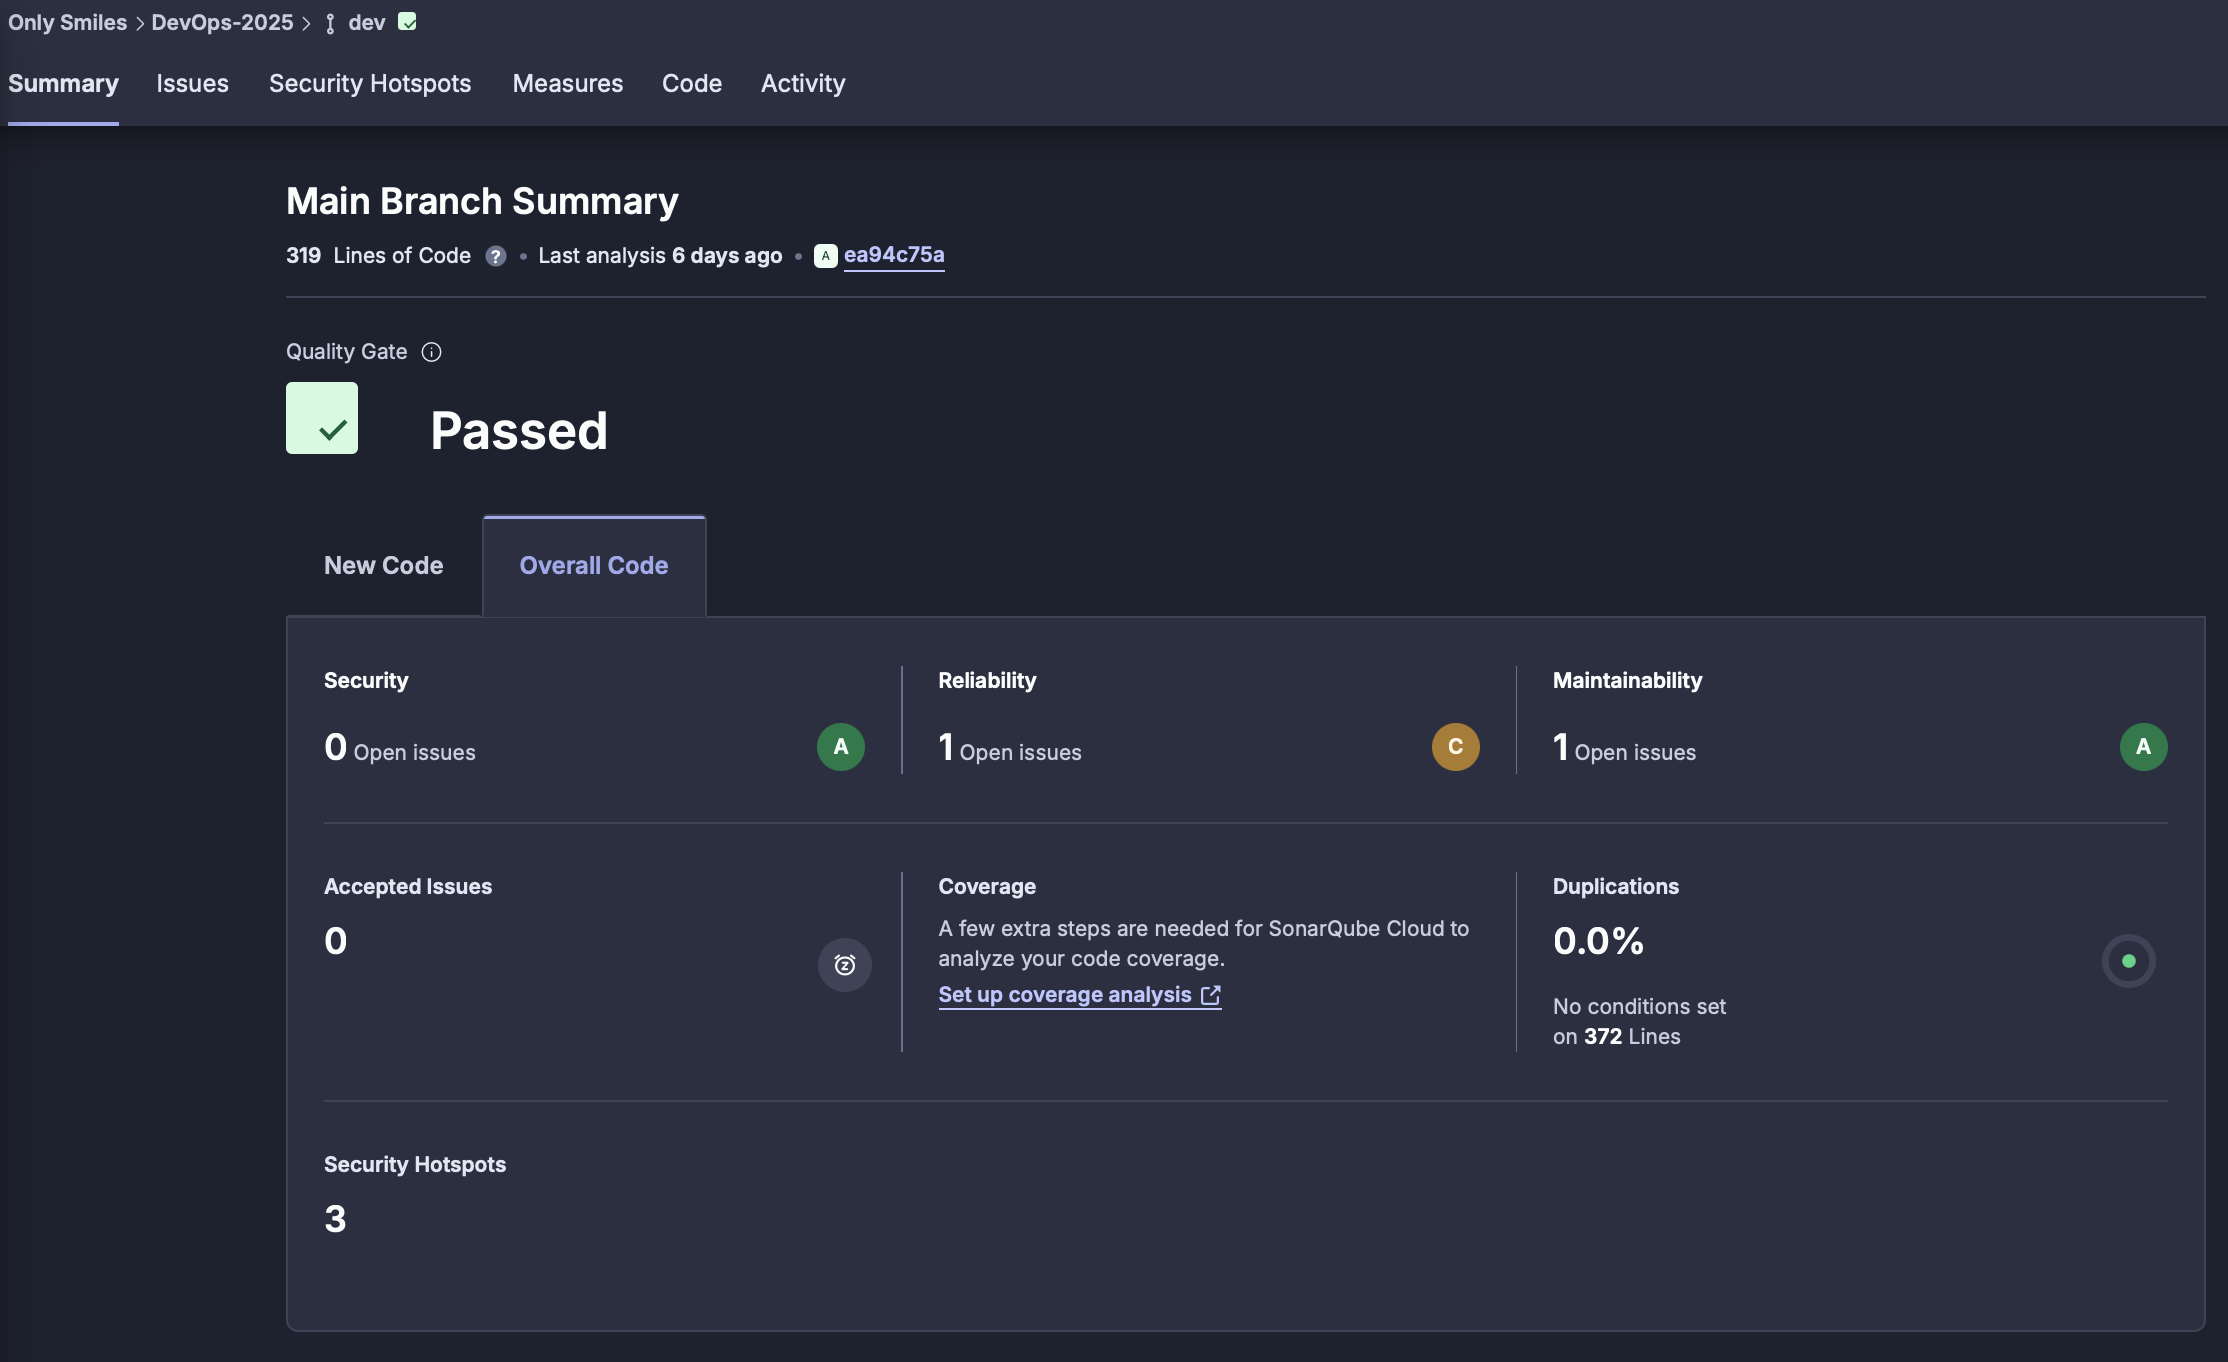
\includegraphics[width=0.8\textwidth]{images/sonarcube-report.png} \\
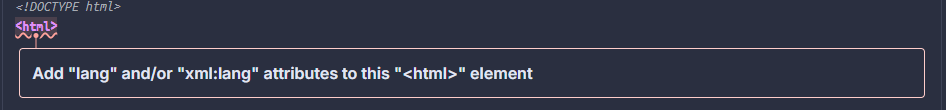
\includegraphics[width=0.8\textwidth]{images/sonarcube_relaibility_issue.png}\\
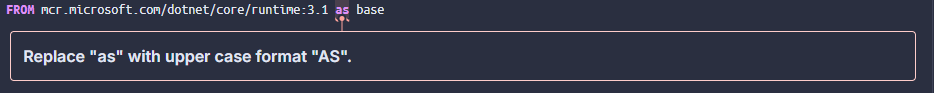
\includegraphics[width=0.8\textwidth]{images/sonarcube_maintainability_issue.png}\\
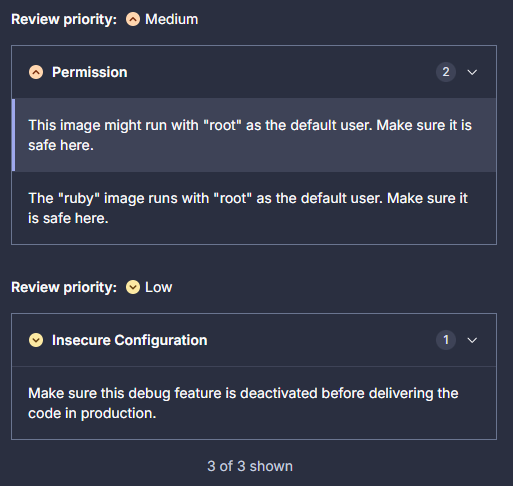
\includegraphics[width=0.6\textwidth]{images/sonarcue_security_hotspots.png}

\newpage
\subsection{Security Assesment - already enforced practices}\label{appendix:security}

The VMs hosted on DigitalOcean droplets are only accessible via SSH. Public SSH keys are added through the DigitalOcean UI, ensuring that only authorized developers with the corresponding private keys can connect. Furthermore, we made use of DigitalOcean Space and GitHub Secrets to securely store our environment variables and sensitive configuration values, such as API keys and credentials, separating them from our codebase. This minimizes the risk of accidental exposure.

To secure communication between users and our servers, we configured DNS for our domain and enabled HTTPS using TLS certificates. This ensures that all transmitted data is encrypted and protected against interception and Man-in-the-Middle attacks.

For database security, we moved our database to a private internal network, making it inaccessible from the public internet.

Finally, we enhanced credential security by using autogenerated strong passwords for all service accounts and system users. This reduces the likelihood of successful brute-force attacks and improves overall system resilience.

